% Full instructions available at:
% https://github.com/elauksap/focus-beamertheme

\documentclass{beamer}
\usetheme[numbering=progressbar]{focus}
\usepackage{tikz}
\usetikzlibrary{positioning}
\usetikzlibrary{shapes,arrows}
\usepackage{transparent}
\usepackage{fancyvrb}
\usepackage{listings}
\definecolor{main}{RGB}{47, 161, 219}
%\definecolor{textcolor}{RGB}{128, 128, 128}
\definecolor{background}{RGB}{240, 247, 255}
\definecolor{textcolor}{RGB}{85, 87, 83}
\title{D4 Project}
\subtitle{Passive DDoS identification techniques}
\author{TEAM CIRCL}
\titlegraphic{\includegraphics[scale=0.20]{d4-logo.pdf}}
\institute{Team CIRCL \\ \url{https://www.d4-project.org/}}
\date{20190329}

\begin{document}
    \begin{frame}
        \maketitle
    \end{frame}


\begin{frame}
\frametitle{Observing SYN floods attacks in backscatter traffic}
Attack description

    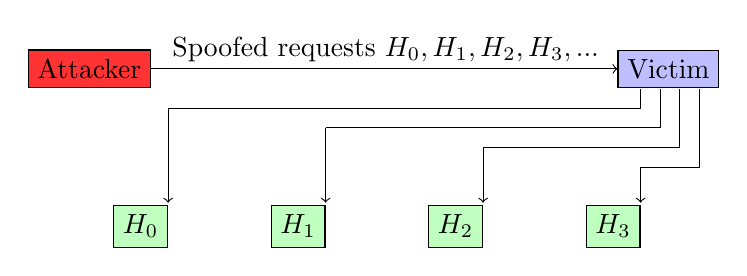
\begin{tikzpicture}{scale=0.4}
    \node[rectangle,draw,fill=red!80] (a) at (0,0) {Attacker};
    \node[anchor=west] at (0.93,0.25) {Spoofed requests $H_{0},H_{1},H_{2},H_{3},...$};
    \node [rectangle,draw,fill=blue!25,anchor=east] at (8,0) (v) {Victim};
    \draw [->](a) --(v);

    \foreach \x in {0,1,2,3} {
        \node [rectangle,draw,fill=green!25,anchor=east] at (\x*2+1,-2) {$H_{\x}$};
        %Horizontal lines
        \draw (\x*2+1, -\x*0.25-0.5)--(7.0+\x*.25,-\x*0.25-0.5);
        %Links to the victim
        \draw (7.0+\x*.25,-\x*0.25-0.5) -- (7.0+\x*.25,-0.25);
        %Links to hosts
        \draw[->] (\x*2+1, -\x*0.25-0.5)--(\x*2+1,-1.70);
    }
    \end{tikzpicture}


\begin{center}
    \begin{tabular}{|l|}
        \hline
        Connections\\
        \hline
        $H_{0}$\\
        \hline
        $H_{1}$\\
        \hline
        $H_{2}$\\
        \hline
        $H_{3}$\\
        \hline
    \end{tabular}
\end{center}

\begin{center}
Fill up state connection state table of the victim
\end{center}

\end{frame}

\begin{frame}
\frametitle{How does backscatter look like?}
\input{tcpout.tex}
\begin{center}
    \alert{What are the typical characteristics?}
\end{center}
\end{frame}

\begin{frame}
\frametitle{What can be derived from backscatter traffic?}

\begin{itemize}
    \item External point of view on ongoing denial of service attacks
    \item Confirm if there is a DDOS attack
    \item Recover time line of attacked targets
    \item Confirm which services (DNS, webserver, $\dots$)
    \item Infrastructure changes
    \item Assess the state of an infrastructure under denial of service attack
    \begin{itemize}
        \item Detect failure/addition of  intermediate network equipments, firewalls, proxy servers etc
        \item Detect DDOS mitigation devices
    \end{itemize}
    \item Create probabilistic models of denial of service attacks
\end{itemize}
\end{frame}

\begin{frame}
    \frametitle{Confirm if there is a DDOS attack}
    \begin{block}{Problem}
        \begin{itemize}
            \item Distinguish between compromised infrastructure and backscatter
            \item Look at TCP flags $\to$ filter out single SYN flags
            \item Focus on ACK, SYN/ACK, ...
            \item Do not limit to SYN/ACK or ACK $\to$ ECE (ECN Echo)\footnote{\url{https://tools.ietf.org/html/rfc3168}}
        \end{itemize}
    \end{block}
    \input{flags.tex}
\end{frame}

\begin{frame}
    \frametitle{Observing SYN floods attacks in backscatter traffic}
    Plotting TCP acknowledgement numbers
    \begin{center}
        \scalebox{0.7}{\input{backscatter.tex}}
    \end{center}
\end{frame}

\begin{frame}
\frametitle{Get in touch if you want to join the project, host a sensor or contribute}
\begin{itemize}
\item Collaboration can include research partnership, sharing of collected streams or improving the software.
\item Contact: info@circl.lu
\item \url{https://github.com/D4-Project} -  \url{https://twitter.com/d4_project}
\end{itemize}
\end{frame}


\end{document}
